\subsection{Graphs and graph convolutions}

Graphs are sets of nodes connected by edges, as shown in Fig.~\ref{fig:graph_example}

\begin{figure}[H]
	\centering
	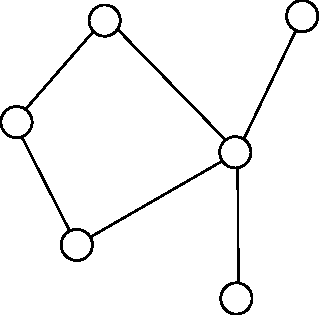
\includegraphics[width=0.4\columnwidth]{img/graph_example.pdf}
	\caption{Example graph where nodes are individuals and edges are their contacts at time step $t$.}
	\label{fig:graph_example}
\end{figure}

We model partially infected populations as a graph, where each individual (interchangeably called agent) is a node. Edges of this graph model contacts between two agents. The dynamics of infections throughout the population is described by graph convolutions. The definition of a graph convolution~\cite{Kipf2017SemiSupervisedCW} for here is

\begin{equation}
	\label{eq:graph_convolution}
	h_{v_i}^{(l+1)} = \sum_{j\in A(i)} h_{v_j}^{(l)}
\end{equation}

with $h_{v_i}^{(l)}$ denoting the feature vector of node $i$ of iteration $(l)$ and $A(i)$ as all neighbours of node $i$ as described by the adjacency matrix $A$. This formulation is equivalent to the matrix formulation $h^{(l+1)} = A h^{(l)}$ with $A$ as adjacency matrix as shown in \ref{sec:consistency}. We consider here adjacency matrices without diagonal elements.

Each agent $i$ is modeled by $D$ features, $h_{v_i} \in \mathbb{R}^D$. Therefore, the feature matrix, $h^{(l)}$, consists of all agents' features at time $(l)$ and is thereby of dimension $N\times D$ where there are $N$ agents in the population and each agent is described by $D$ features. A three dimensional feature space is used in this work, $D=3$, modeling three possible health states. The unit vectors of this space are interpreted as following:
\begin{itemize}
	\item $\vec{e}_0$: susceptible state
	\item $\vec{e}_1$: infected state
	\item $\vec{e}_2$: recovered state
\end{itemize}
A uniform distribution over these possible states expresses complete uncertainty of the health state of an agent.

\subsection{SIR Model}
Our basic stochastic SIR model relies on the assumptions that every person in an environment can be modeled as a point value on a grid, which has a location (i.e.\ GPS coordinates) and an infection state. These states can be either \textit{susceptible} (S), \textit{infected} (I), \textit{recovered} (R) or in advanced models also \textit{under quarantine} (Q) or \textit{dead} (D). All individuals, here called agents, have a probability (here called diffusion rate $d$) to make a step on the grid per time step on a predefined grid. The movement is a random walk pattern. In the case that some agents meet at the same location, disease spreading can occur. An infected agent spreads the disease with the probability $\beta$ to all the agents in its close vicinity (same location on the grid). Furthermore, recovery is covered by taking a recovery rate into account, i.e.\ a probability $\gamma$ to recover from the disease per time step. If an infected agent recovers from the disease, the state of the agent changes from \textit{infected} to \textit{recovered}, which is definite (no double infections). The process ends, when no infected agents are left. For more background the reader is reffered to \cite{weiss2013sir} and \cite{epstein2009modelling}.

